%! Author = breandanconsidine
%! Date = 7/19/21

% Preamble
\documentclass[mathserif,notheorems]{beamer}

% Packages
\usepackage{fontspec}
\usepackage{amsmath}

% https://tex.stackexchange.com/a/34486/139648
\usepackage{tikz}
\usetikzlibrary{calc}
\newcommand{\tikzmark}[1]{\tikz[overlay,remember picture] \node (#1) {};}

\usepackage[pdf]{graphviz}
\usepackage{amssymb}
\usepackage{mathrsfs}
\usepackage{xcolor}
\usepackage{pifont}% http://ctan.org/pkg/pifont
\newcommand{\cmark}{\color{green}\ding{51}}%
\newcommand{\xmark}{\color{red}\ding{55}}%

\usepackage{blkarray}% http://www.hss.caltech.edu/~kcb/TeX/kbordermatrix.sty


% https://tex.stackexchange.com/a/285558/139648
\usepackage{amsthm}
\setbeamertemplate{theorems}[numbered] % to number

\theoremstyle{plain} % insert bellow all blocks you want in italic
\newtheorem{theorem}{Theorem}[section] % to number according to section

\theoremstyle{definition} % insert bellow all blocks you want in normal text
\newtheorem*{definition}{Definition} % to number according to section
\newtheorem*{idea}{Proof idea} % no numbered block

\usepackage{graphicx}
\usepackage{tcolorbox}
% ---------

\title{\href{https://arxiv.org/pdf/2106.06981.pdf}{Thinking Like Transformers}}
\subtitle{Gail Weiss, Yoav Goldberg, Eran Yahav}

\author{Presented by Breandan Considine}

\institute[McGill]{
  McGill University \\
  \medskip
  \textit{breandan.considine@mail.mcgill.ca}
}
\date{\today}

% Document
\begin{document}
  \begin{frame}
    \titlepage
  \end{frame}


  \begin{frame}
    \frametitle{How does a transformer think, intuitively?}
    \begin{tcolorbox}
    Intuitively, transformers’ computations are applied to their
    entire input in parallel, using attention to draw on and combine tokens from several positions at a time as they make
    their calculations (Vaswani et al., 2017; Bahdanau et al.,
    2015; Luong et al., 2015). The iterative process of a transformer is then not along the length of the input sequence but
    rather the depth of the computation: the number of layers it
    applies to its input as it works towards its final result.
      \begin{flushright}
        --Weiss, Goldberg \& Yahav
      \end{flushright}
    \end{tcolorbox}
  \end{frame}

  \begin{frame}
    \frametitle{What purpose does the RASP language serve?}

    \begin{tcolorbox}
      We find RASP a natural tool for conveying transformer
      solutions to [\ldots] tasks for which a human can encode a solution: we do not
      expect any researcher to implement, e.g., a strong language
      model or machine-translation system in RASP\ldots we
      focus on programs that convey concepts people can
      encode in ``traditional'' programming languages, and the
      way they relate to the expressive power of the transformer\ldots\\

      Considering computation problems and their implementation in RASP allows us to “think
      like a transformer” while abstracting away the technical
      details of a neural network in favor of symbolic programs.

      \begin{flushright}
        --Weiss, Goldberg \& Yahav
      \end{flushright}
    \end{tcolorbox}
  \end{frame}

  \begin{frame}
    \frametitle{RASP: Restricted Access Sequence Processing}
    If transformers are a series of operators applied to an input sequence in parallel, what operations could they be performing?\linebreak

    Not saying transformers are RASPs, but \textit{for problems with known solutions}, they often share a curiously similar representation\ldots\linebreak

    How do we do pack useful compute into matrix/vector arithmetic? Array programming seems to be a surprisingly good fit.\linebreak

    \begin{itemize}
      \item Data types: $\{\mathbb{R, N, B}, \Sigma\}^n, \mathbb{B}^{n\times n}$
      \item Elementwise ops: $\{+, \times, \texttt{pow}\}: \mathbb{N}^n \rightarrow \mathbb{N}^n$ (e.g. $\mathbf{x} + \mathbf{1}$)
      \item Predicates: $\{\mathbb{R, N}, \Sigma\}^n → \mathbb{B}^n$
      \item Standard functions: \texttt{indices}$:\Sigma^n→\mathbb{N}^n$, \texttt{tokens}$:\mathbb{N}^n→\Sigma^n$,
    \end{itemize}
  \end{frame}

  \begin{frame}
    \frametitle{Selection operator}
    Takes a key, query and predicate, and returns a selection matrix: \\

      $$
      \texttt{select}: \big(\underbrace{\mathbb{N}^n}_{key} \times \underbrace{\mathbb{N}^n}_{query} \times \underbrace{(\mathbb{N} \times \mathbb{N} \rightarrow \mathbb{B})}_{predicate}\big)\rightarrow \mathbb{B}^{n\times n}
      $$

    \noindent\rule{\textwidth}{1pt}
    \begin{align*}
        \texttt{select(}\underbrace{[\tikzmark{a}0, \tikzmark{b}1, \tikzmark{c}2]}_{key},
        \underbrace{\begin{bmatrix}
          1 \\
          2 \\
          3
        \end{bmatrix}
        }_{query}, <\texttt{)}
        &=
        \begin{blockarray}{cccc}
          & \tikzmark{d}0 & \tikzmark{e}1 & \tikzmark{f}2 \\
          \begin{block}{c[ccc]}
            1 & 0 < 1 & 1 < 1 & 2 < 1 \\
            2 & 0 < 2 & 1 < 2 & 2 < 2 \\
            3 & 0 < 3 & 1 < 3 & 2 < 3
          \end{block}
        \end{blockarray}\\
        &=
        \begin{bmatrix}
          \textbf{T} & F & F \\
          \textbf{T} & \textbf{T} & F \\
          \textbf{T} & \textbf{T} & \textbf{T}
        \end{bmatrix}
        \end{align*}
    \end{frame}

    \begin{frame}
      \frametitle{Aggregate}
      Takes a selection matrix, a list, and averages the selected values:\\
      $$
      \texttt{aggregate}: (\mathbb{B}^{n\times n} \times \underbrace{\mathbb{N}^n}_{list}) → \mathbb{R}^n
      $$
        \noindent\rule{\textwidth}{1pt}
    \begin{align*}
        \texttt{aggregate(}\begin{bmatrix}
        \textbf{T} & F & F \\
        \textbf{T} & \textbf{T} & F \\
        \textbf{T} & \textbf{T} & \textbf{T}
      \end{bmatrix},
      \begin{bmatrix}
        10 & 20 & 30
      \end{bmatrix}\texttt{)}
      &=
      \begin{bmatrix}
        \frac{10}{1} & \frac{10 + 20}{2} & \frac{10 + 20 + 30}{3}
      \end{bmatrix}\\
      &=
      \begin{bmatrix}
        10 & 15 & 20
      \end{bmatrix}
      \end{align*}
  \end{frame}

  \begin{frame}
    \frametitle{Selector width}
    Takes a selection matrix, a string and returns the histogram:
    $$
    \texttt{selector\_width}: \mathbb{B}^{n\times n} → \Sigma^n → \mathbb{N}^n
    $$
    \noindent\rule{\textwidth}{1pt}
    \begin{align*}
      &\texttt{selector\_width(same\_token)(}
      \begin{bmatrix}
        \texttt{h} & \texttt{e} & \texttt{l} & \texttt{l} & \texttt{o}
      \end{bmatrix}\texttt{)}\\
      &=
      \begin{bmatrix}
        \textbf{T} & F & F & F & F \\
        F & \textbf{T} & F & F & F \\
        F & F & \textbf{T} & \textbf{T} & F \\
        F & F & \textbf{T} & \textbf{T} & F \\
        F & F & F & F & \textbf{T} \\
      \end{bmatrix}
      \begin{bmatrix}
        \texttt{h} & \texttt{e} & \texttt{l} & \texttt{l} & \texttt{o}
      \end{bmatrix}\\
      &=
      \begin{bmatrix}
        1 & 1 & 2 & 2 & 1
      \end{bmatrix}
    \end{align*}
  \end{frame}

  \begin{frame}
    \frametitle[short frame title]{Dyck words and languages}
    \begin{tcolorbox}
      \begin{definition}

        A \textbf{Dyck-1 word} is a string containing the same number of ('s and )'s, where the number of )'s in every prefix is less than or equal to the number of ('s.
      \end{definition}
    \end{tcolorbox}

    \begin{itemize}
      \item[\cmark]\texttt{((())), (())(), ()(()), (()()), ()()()}
      \item[\xmark]\texttt{)))(((, ))(()(, )())((, ))()((, )()()(, ((()(),\ldots}
    \end{itemize}

    \begin{tcolorbox}
      \begin{definition}
        A \textbf{Dyck-n word} is a Dyck word with n bracket types.
      \end{definition}
    \end{tcolorbox}

    \begin{itemize}
      \item[\cmark]\texttt{()[]\{\}, ([]\{\}), [()\{\}], \{()[]\}, ([])\{\}, [()]\{\}, \ldots}
      \item[\xmark]$\underbrace{\texttt{([)]\{\}, [\{]\}(),  [\{](\}), ([)\{]\}, } \ldots}_{\text{shuffle Dyck-3}}$ \texttt{, \}\{()]]}
    \end{itemize}
  \end{frame}

  \begin{frame}
    \frametitle{Experiments}
    Three sets of experiments:
    \begin{itemize}
      \item With attention supervision: assuming the solution could be learned, would it even work in the first place?
      \item Without attention supervision: does standard supervision (i.e. cross-entropy loss on the target without teacher forcing) recover the same (or similar) solution?
      \item How tight are the RASP-implied bounds for the minimum number of layers and maximum attention heads? Compile the RASP to a transformer: there exists a transformer which can solve the task! But can we recover it via learning?
    \end{itemize}
  \end{frame}

  \begin{frame}
    \frametitle{Experiment #1: Compiling RASP to transformers}
    Can we force a transformer to implement RASP selectors?
    \begin{center}
      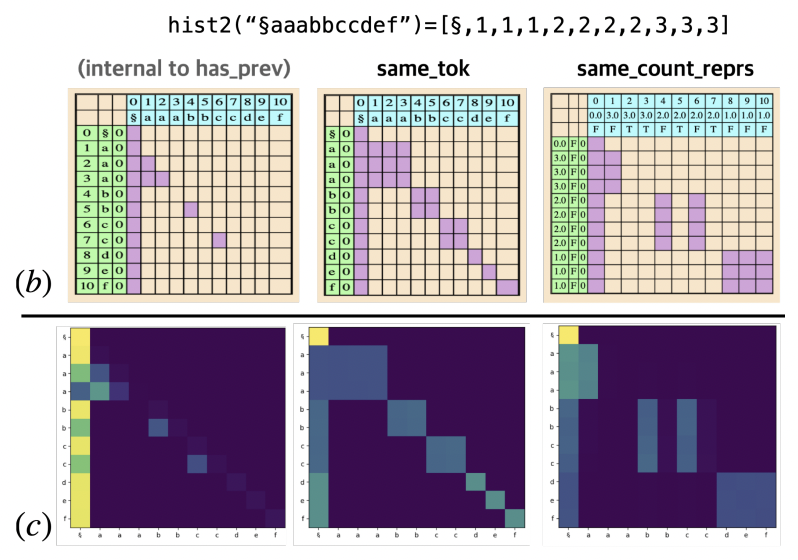
\includegraphics[scale=0.6]{rasp_vs_attention}
    \end{center}
  \end{frame}

  \begin{frame}
    \frametitle{Experiment #2: Can it be learned / does it learn the same thing?}
    So there exists a feasible solution. Can it be learned from scratch?
    \begin{center}
      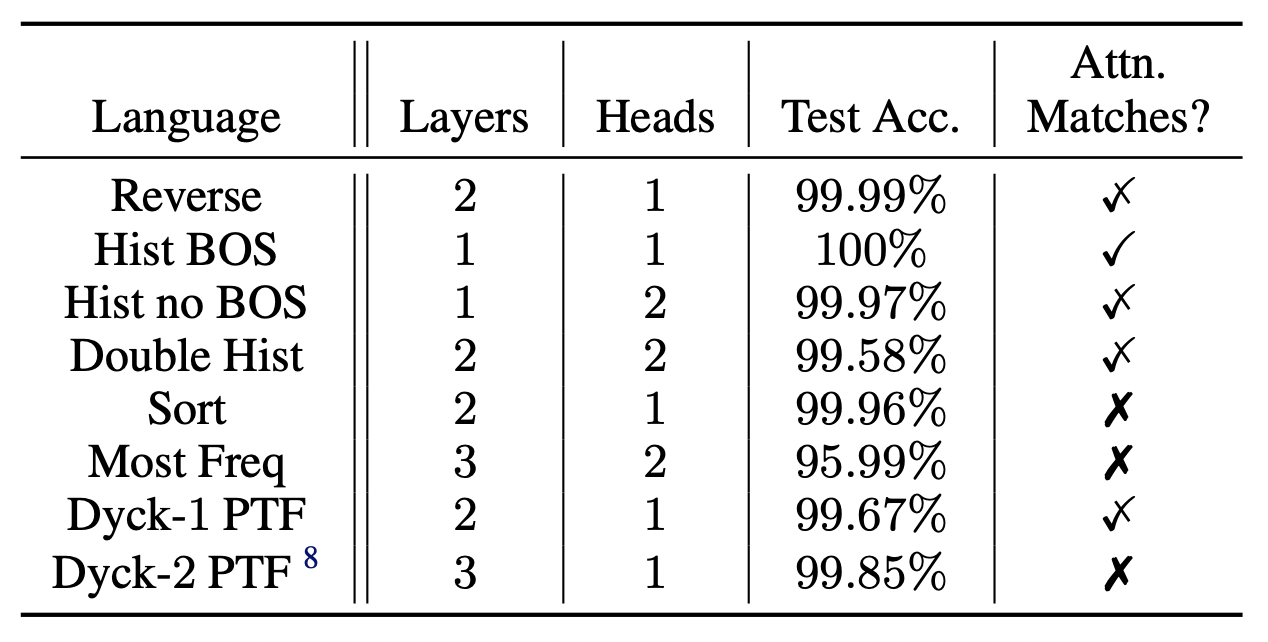
\includegraphics[scale=0.45]{table1}
    \end{center}
  \end{frame}


  \begin{frame}
    \frametitle{Experiment #3: How tight are the L, H bounds?}
    Is the RASP-implied depth/width necessary and/or sufficient?
    \begin{center}
      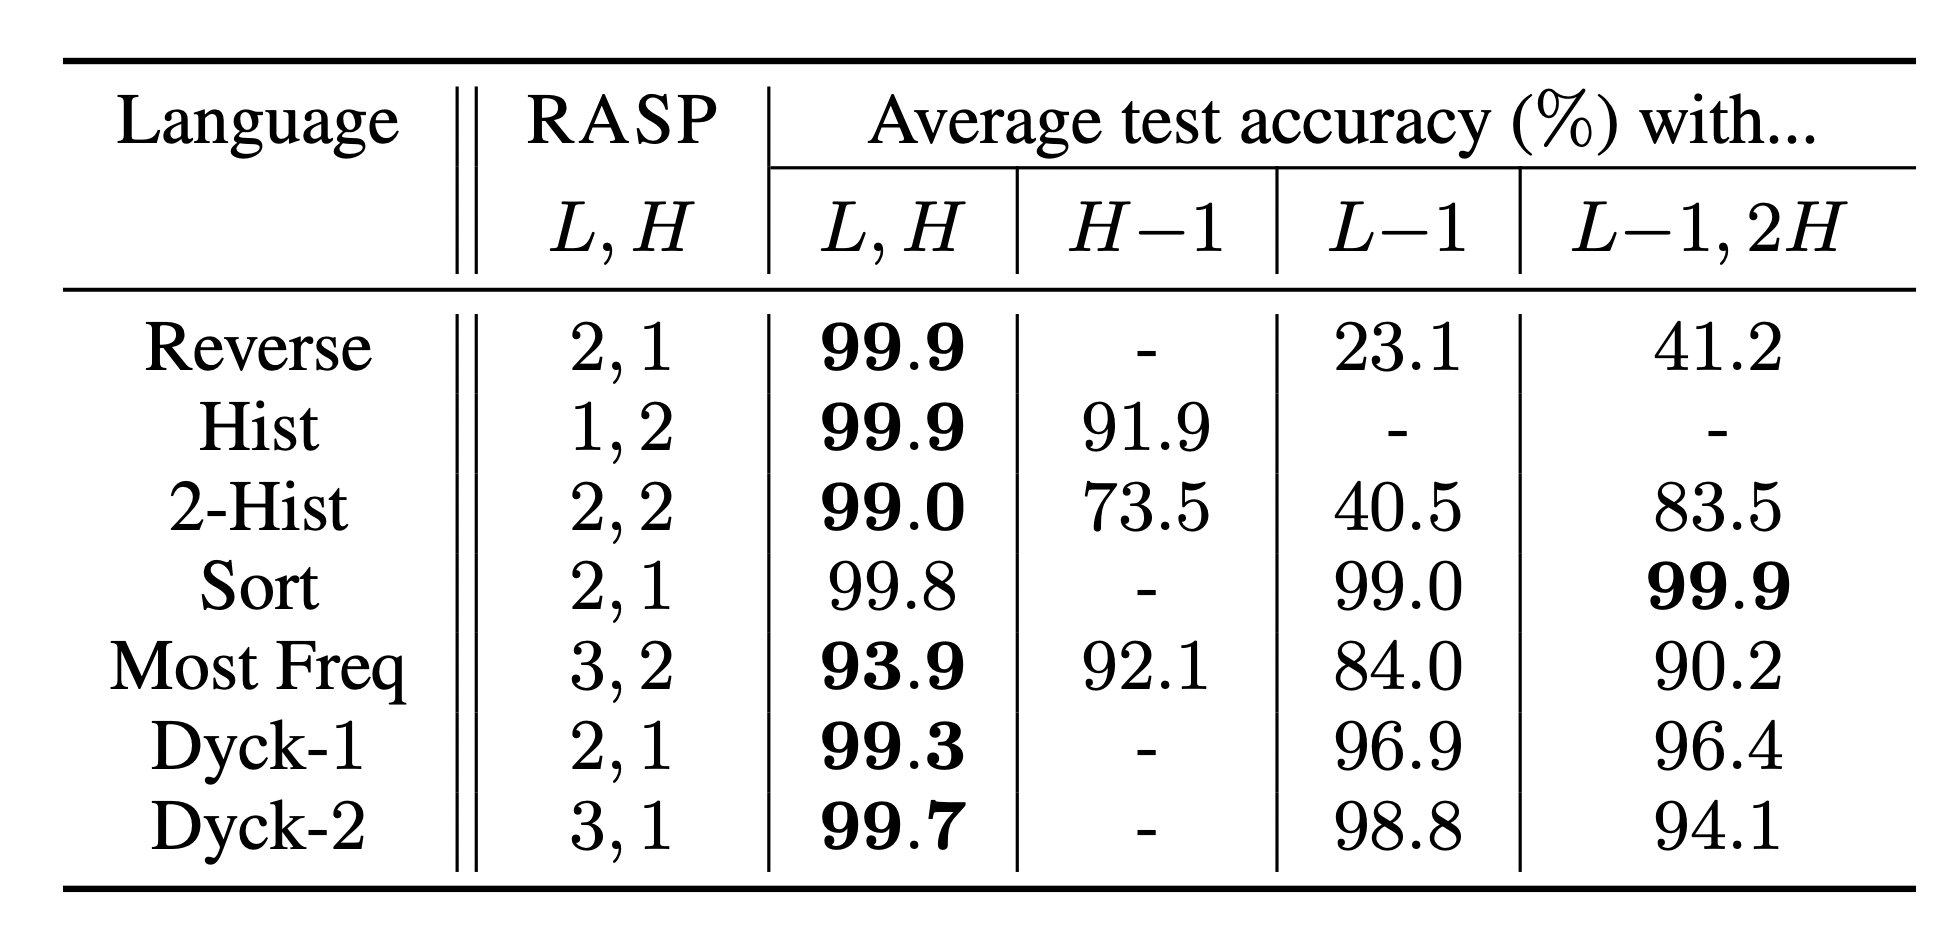
\includegraphics[scale=0.3]{table2}
    \end{center}
  \end{frame}

  \begin{frame}
    \frametitle{What is this paper trying to say?}
    \begin{itemize}
      \item Array programming provides an intuitive model for thinking about transformer reasoning
      \item Can logical matrices be interpreted as the fixed points of self attention (for certain problems)?
      \item The [optimal?] RASP solution a human constructs often matches the solution a transformer discovers
      \item Given a known solution, we can predict sufficient hyperparameters (e.g. depth, width) needed to learn it
    \end{itemize}
  \end{frame}

  \begin{frame}
    \frametitle{Threats to validity}
    \begin{itemize}
      \item How do we know whether RASP solutions are learnable? What do the L, H bounds tell us?
      \item Do transformers really think this way? Or are we just selecting problems which we can force a transformer to reproduce that are relatively ``learnable''?
      \item Are there ``unlearnable'' tasks for which the RASP-implied bounds do not predict learnability in practice?
      \item What other evidence could be shown to demonstrate transformers actually think this way?
      \item What does these results really mean if we need to know a RASP solution exists a priori? If we knew it to begin with, would we really need a transformer to find it?
      \item Still, not a huge leap to think, \textit{if} a human solution might exist and could be learned, maybe it could be decoded\ldots
    \end{itemize}
  \end{frame}

  \begin{frame}
    \frametitle{Unanswered questions/Future work}
    \begin{itemize}
      \item How does ordering work? If selectors can be merged, how do you align attention heatmaps with selectors?
      \item What can we say (if anything) about uniqueness? Is there a way to canonicalize attention/selector order?
      \item Is there a way to ``scale up'' to longer sequences? How do/can you ``upsample'' a RASP heatmap?
      \item Would it be possible to extract RASP source code from a pretrained transformer?
      \item What other evidence could be shown to demonstrate transformers actually think this way?
    \end{itemize}
  \end{frame}

  \begin{frame}
    \frametitle{References on Formal Language Induction / Recognition}
    \begin{itemize}
      \item Weiss et al., \href{https://arxiv.org/pdf/2009.11264v2.pdf}{Thinking Like Transformers} (2021)
      \item Weiss et al., \href{https://arxiv.org/pdf/1805.04908.pdf}{On the Practical Computational Power of Finite Precision RNNs for Language Recognition} (2018)
      \item Weiss et al., \href{https://arxiv.org/pdf/1910.13895.pdf}{Learning Deterministic Weighted Automata with Queries and Counterexamples} (2019)
      \item Weiss et al., \href{http://proceedings.mlr.press/v80/weiss18a/weiss18a.pdf}{Extracting Automata from Recurrent Neural Networks
      Using Queries and Counterexamples} (2018)
      \item Bhattamishra et al., \href{https://arxiv.org/pdf/2009.11264v2.pdf}{On the Ability and Limitations of Transformers to Recognize Formal Languages} (2020)
      \item Bhattamishra et al., \href{https://arxiv.org/pdf/2011.03965.pdf}{On the Practical Ability of Recurrent Neural Networks to Recognize Hierarchical Languages} (2020)
    \end{itemize}
  \end{frame}

\end{document}

